\section*{Question 4:}
Exercise 10.8:

Implement the nearest neighbor–based collaborative filtering algorithm. Using a publicly available collaborative filtering data set, compare the effectiveness, in terms of mean squared error, of the Euclidean distance and correlation similarity.

\subsection*{Answer:}
I implemented the nearest neighbor-based collaborative filtering algorithm in python and saved it in the file nn.py. It takes one command line argument, which is the ratings file in csv format. The program computes MSE of Euclidean distance and correlation similarity.

\lstinputlisting[language=python, label=nn.py, caption=The content of nn.py, breakatwhitespace=〈false)]{Q4/nn.py}


\textbf{Results:}

\begin{figure}[h]
\caption{Running nn.py}
\centering
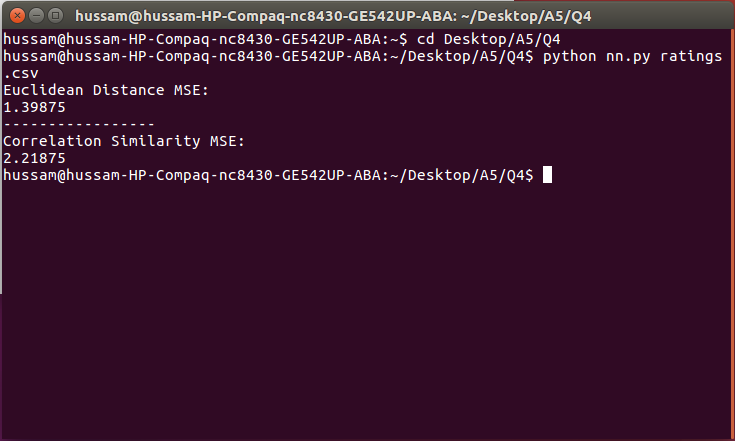
\includegraphics[scale=0.45]{Q4/nn.png}
\end{figure}

The MSE of Euclidean distance is smaller than the MSE of the correlation similarity. Therefore the Euclidean distance is more effective than correlation similarity.
